\documentclass[10pt]{beamer}
\usepackage[utf8]{inputenc}

\usetheme{metropolis}
\usepackage{appendixnumberbeamer}

\usepackage{booktabs}
\usepackage[scale=2]{ccicons}
\usepackage{graphicx}
\usepackage{pgfplots}
\usepackage{tikz}
% \usepackage{hhline}
\usetikzlibrary{shapes.geometric, positioning, arrows.meta}
\usepgfplotslibrary{dateplot}

\usepackage[dvipsnames]{xcolor}
\usepackage{xcolor}
\usepackage{colortbl}
\usepackage{tabularx}

\usepackage{xspace}
\newcommand{\themename}{\textbf{\textsc{metropolis}}\xspace}


\definecolor{CanvasBG}{HTML}{FAFAFA}

% From the official style guide
\definecolor{UnccGreen}{HTML}{005035}
\definecolor{UnccLightGreen}{HTML}{C3D7A4}
\definecolor{UnccGold}{HTML}{c1d7fe}
\definecolor{UnccOrange}{HTML}{F3901D}
\definecolor{UnccLightYellow}{HTML}{899064}
\definecolor{UnccBlue}{HTML}{007377}
\definecolor{UnccPink}{HTML}{DE3A6E}
\definecolor{White}{HTML}{FFFFFF}
\definecolor{LightGray}{HTML}{F1E6B2}
\definecolor{Purple}{HTML}{6c5098}
\definecolor{Bordeau}{HTML}{570514}
\definecolor{ULB_blue}{HTML}{003087}

\setbeamercolor{frametitle}{bg=ULB_blue}
\setbeamercolor{progress bar}{bg=UnccGold, fg=ULB_blue}
\setbeamercolor{alerted text}{fg=UnccOrange}

\setbeamercolor{block title}{bg=UnccGreen, fg=White}
\setbeamercolor{block title example}{bg=UnccBlue, fg=White}
\setbeamercolor{block title alerted}{bg=UnccPink, fg=White}
\setbeamercolor{block body}{bg=LightGray}

\metroset{titleformat=smallcaps}

% progressbar=foot}

\makeatletter
\setlength{\metropolis@progressinheadfoot@linewidth}{2pt}
\setlength{\metropolis@titleseparator@linewidth}{2pt}
\setlength{\metropolis@progressonsectionpage@linewidth}{2pt}




% \title{Présentation de mi-parcours mémoire}
\subtitle{Étude de spectres infrarouges de géantes rouges évoluées}
% \date{\today}
\date{}
\author{\small Margaux Vandererven}
\institute{\small Supervisé par Sophie Van Eck}
 \titlegraphic{\hfill\includegraphics[height=1.5cm]{/Users/margauxvandererven/Documents/unif2023-2024/spectre_IR/rapport/figures/science.png}}

\begin{document}
\maketitle

\begin{frame}[fragile]{Processus s}
    % \begin{columns}
    %     \begin{column}{0.3\textwidth}
    %         +50\% éléments plus lourds que le fer \\
    %     \end{column}
    %     \begin{column}{0.7\textwidth}
    %         \centering
    %         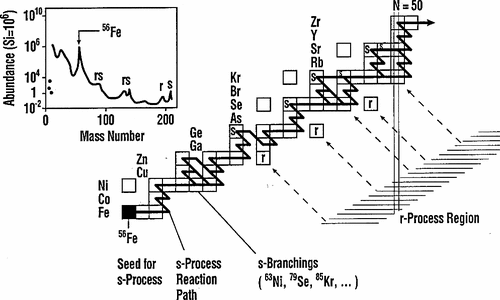
\includegraphics[width=8cm]{images/medium.png}
    %     \end{column}
    % \end{columns}
    \begin{center}
        + de 50\% éléments plus lourds que le fer \\
        $\tau_{\beta^-}$ $<$ $\tau_{\mathrm{n-capture}}$
    \end{center}
    \vfill

    \begin{center}

        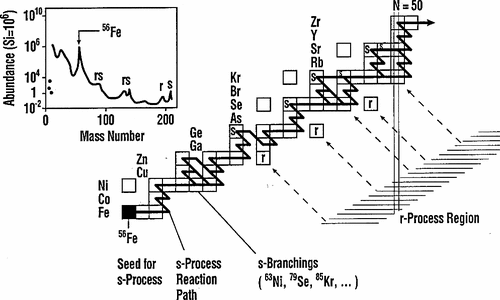
\includegraphics[width=10cm]{images/medium.png} \\
        \end{center}
    \footnotesize{Käppeler et al. 2011.}


\end{frame}

\begin{frame}[fragile]{Étoiles de type S \& étoiles à baryum}

    \begin{columns}
            \begin{column}{0.6\textwidth}

                    T$_{\text{eff}}$ étoiles S $\sim$ T$_{\text{eff}}$ étoiles M\\

                    Bandes ZrO \& enrichissement en éléments s
    

    					\begin{itemize}
    						\item de type S intrinsèques (Tc rich) 
                            \begin{tikzpicture}[remember picture,overlay]
                                \draw[->,thick,black] (current page.center) +(0.,0.7) -- +(1.5,1) 
                                    node[midway,right] {};
                            \end{tikzpicture}
    						\item de type S extrinsèques (Tc poor)
                            \begin{tikzpicture}[remember picture,overlay]
                                \draw[->,thick,black] (current page.center) +(0.,0.1) -- +(1.,-0.4) 
                                    node[midway,right] {};
                            \end{tikzpicture}
    						\item[] 
    					\end{itemize} 
                        \vspace{0.5cm}

                        T$_{\text{eff}}$ étoiles à baryum $\sim$ T$_{\text{eff}}$ étoiles G-K\\
                        Enrichissement en éléments s \\
                        % Extrinsèques en sytème binaire.
            \end{column}
            \begin{column}{0.4\textwidth}
                \centering
                \includegraphics[width=\textwidth]{/Users/margauxvandererven/Documents/unif2023-2024/spectre_IR/rapport/figures/agb_structure.jpeg}
    			\footnotesize{\textit{Structure interne d'une étoile AGB.} (Persson 2014)} \\
                \vspace{0.5cm}
                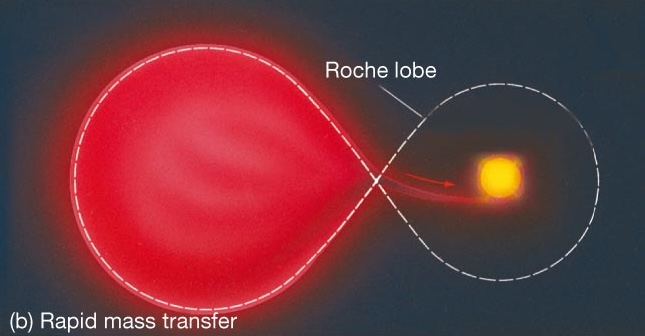
\includegraphics[width=\textwidth]{images/20_22_Figure_Anno.jpg}
                \footnotesize{\textit{Transfert de masse.} (Pearson Education 2014)}
            \end{column}
    \end{columns}
\end{frame}


\begin{frame}[fragile]{Intérêt du travail}
%     % q? de recherche
%     % spectre observé vis et IR
    \begin{columns}
        \begin{column}{0.45\textwidth}
            Beaucoup d'incertitude sur les processus de production des éléments s, ainsi que sur leur détermination d'abondance (jusqu'à $\pm$0.3 dex dans le visible). \\
            \vspace{0.5cm}
            Infrarouge : continu plus atteint, moins de blend à cause des raies moléculaires. \\
            \vspace{0.5cm}
            \textbf{$\rightarrow$} \\
            \textbf{Comparaison visible/infrarouge des paramètres stellaires et abondances.}
        \end{column}  
        \begin{column}{0.55\textwidth}
            \begin{center}
            \footnotesize{Spectre visible BD-22$^{\circ}$1742 (4000K)}\\
            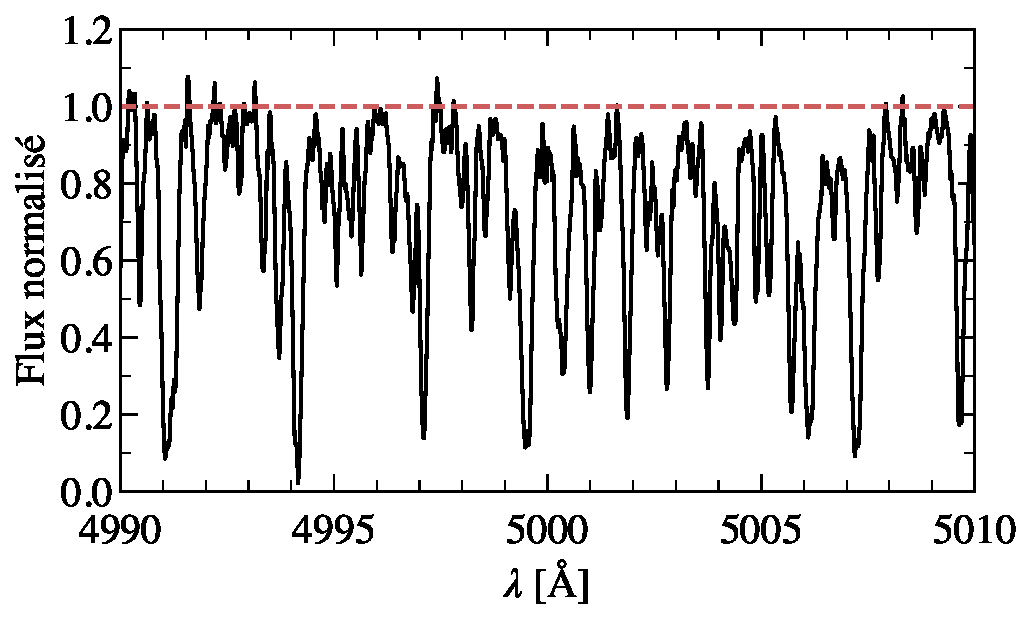
\includegraphics[width=6cm]{images/vis.pdf}\\
            \footnotesize{Spectre IR BD-22$^{\circ}$1742 (4000K)}
            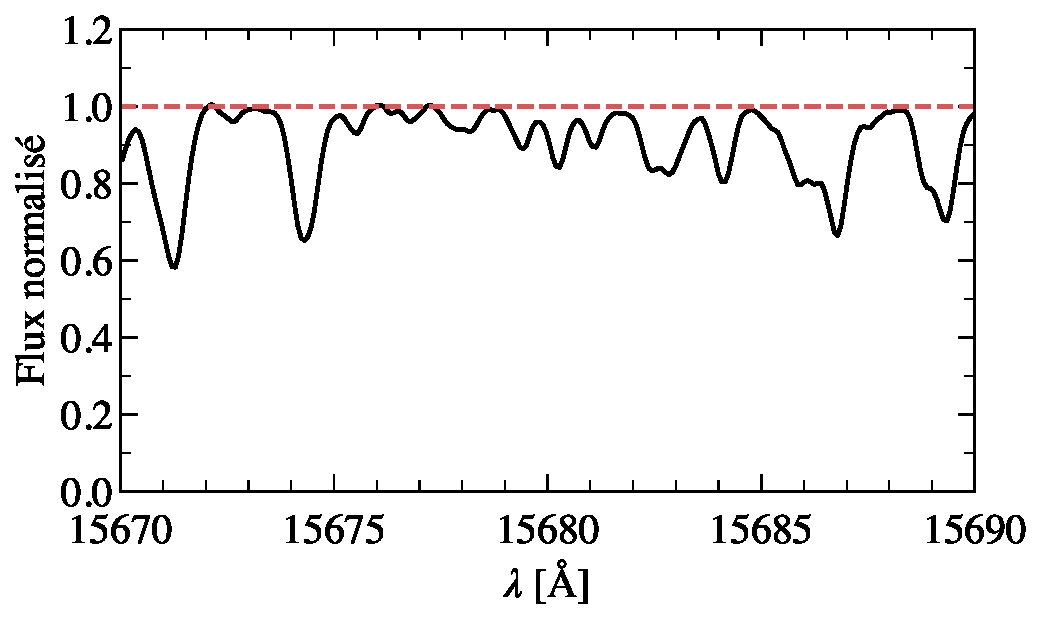
\includegraphics[width=6cm]{images/IR.pdf}\\
            \end{center}
        \end{column}  
    \end{columns}
\end{frame}

\begin{frame}[fragile]{Spectre observé}
% \begin{columns}
%     \begin{column}{0.3\textwidth}
             Spectre infrarouge : \\
             IGRINS (Immersion GRating INfrared Spectrometer) \\ 
             Haute résolution : R=$\frac{\lambda}{\Delta \lambda}$ $\sim$ 45000 \\
    					\begin{itemize}
    						\item Bande H (1.45 - 1.80 $\mu m$)
    						\item Bande K (2.05 - 2.50 $\mu m$)
    						\item[]
    					\end{itemize}
        % $\rightarrow$ BD-2217$^{\circ}$42 (4000K) \\
        \vfill
        \textbf{Correction} : 

        Réduction, correction tellurique, première normalisation par Chris Sneden. 
        
        Seconde normalisation sur pas de 20 Å et correction redshift. \\
%     \end{column}
% \end{columns}
\end{frame}

\begin{frame}[fragile]{Série d'étoiles}
    % \begin{column}{0.7\textwidth}
        \begin{table}[h!]
        %     % \caption{Étoiles et paramètres d'atmosphère stellaire}
                \begin{center}
                \resizebox{\textwidth}{!}{
                \begin{tabular}{cccccc}
                    \hline
                    \hline
                     Étoile & Type spectral & T$_{\rm eff}$ (K) & log $g$ (cm $s^{-2}$) & $\xi_{\rm micro}$ (km s$^{-1}$) & [Fe/H] (dex) \\
                    \hline
                    HD 60197 & K3.5III:Ba3.5 & $3800\pm50^{(3)}$ & $2.00\pm0.50^{(3)}$ & $2.00^{(3)}$ & $-0.60\pm0.20^{(3)}$\\
                    HD 63733 & 	S3.5/3 & $3700^{(1)}$ & $1.00^{(1)}$ & - & $-0.10\pm0.13^{(1)}$ \\
                    CR Cir & S6,2  & - & - & - & - \\
                    HD 123949 & K1pBa & $4378\pm80^{(3)}$ & $1.78\pm0.53^{(3)}$ & $1.37^{(3)}$ & $-0.31\pm0.13^{(3)}$ \\
                    \cellcolor{red!15}BD-22$^{\circ}$1742 & \cellcolor{red!15}S3:*3& \cellcolor{red!15}$4000^{(1)}$ & \cellcolor{red!15}$1.00^{(1)}$ & \cellcolor{red!15}- & \cellcolor{red!15}$-0.30\pm0.09^{(1)}$ \\
                    CD-29$^{\circ}$5912 & S4,4 & $3600^{(4)}$ & $1.00^{(4)}$ & - & $-0.40\pm0.22^{(4)}$ \\
                    BD-18$^{\circ}$2608 & S & $3500^{(2)}$ & $1.00^{(2)}$ & - & $-0.31\pm0.16^{(2)}$ \\
                    HD 116869 & G8III:Ba1 & $4892\pm30^{(3)}$ & $2.59\pm0.07^{(3)}$ & $1.38\pm0.04^{(3)}$ & $-0.44\pm0.09^{(3)}$ \\
                    HD 120620 & K0III (Ba$^{(3)}$) & $4831\pm13^{(3)}$ & $3.03\pm0.30^{(3)}$ & $1.11\pm0.05^{(3)}$ & $-0.30\pm0.10^{(3)}$ \\
                    HD 121447 & K4III$^{(3)}$ (Ba$^{(3)}$) & $4000\pm50^{(3)}$ & $1.00\pm0.50^{(3)}$ & $2.00^{(3)}$ & $-0.90\pm0.13^{(3)}$\\
                    HD 100503 & G/KpBa & $4000\pm50^{(3)}$ & $2.00\pm0.50^{(3)}$ & $2.00^{(3)}$ & $-0.72\pm0.13^{(3)}$ \\
                    HD 119185 &  G8IIIpBa & - & - & - & - \\
                    HD 88562  & K1III (Ba$^{(3)}$)& $4000\pm50^{(3)}$ & $2.00\pm0.50^{(3)}$ & $2.00^{(3)}$ & $-0.53\pm0.12^{(3)}$\\
                    V812 Oph  & S5+/2.5 & $3500^{(2)}$ & $1.00^{(2)}$ & - & $-0.37\pm0.13^{(2)}$\\
                    19 Aql  & F0III-IV & - & - & - & -  \\
                    V915 Aql  & S5+/2 & $3400^{(1)}$ & $0.00^{(1)}$ & - & $-0.50\pm0.15^{(1)}$ \\
                    HD 165774 & S4,6 & - & - & - & - \\
                    \hline
                \end{tabular}}
                \end{center}
        %     % \textbf{Notes}. Le type spectral est majoritairement repris de SIMBAD ; la première lettre faisant référence au système Harvard (O,B,A, F, G, K, M), le chiffre arabe suivant à la nomenclature "early"/"late", le chiffre romain à la classe de luminosité, "Ba" pour étoile à baryum / "S" pour étoile de type S et la lettre minuscule faisant référence aux particularités du spectre (par exemple, "p" pour "particularité non spécifiée").
            
            % \textbf{Références}. $^{(1)}$\cite{shetye_s_2018}, $^{(2)}$\cite{shetye_s_2021} , $^{(3)}$\cite{karinkuzhi_when_2018}, $^{(4)}$\cite{shetye_observational_2019}.
            \footnotesize{\textbf{Références}. $^{(1)}$Shetye et al. 2018, $^{(2)}$Shetye et al. 2021 , $^{(3)}$Karinkuzhi et al. 2018, $^{(4)}$Shetye et al. 2019}
        %     %     \label{param_stellaire}
            \end{table}
    % \end{column}
\end{frame}

\begin{frame}[fragile]{Spectre synthétique}
    \begin{columns}
        \begin{column}{0.48\textwidth}
            \begin{center}
                \textbf{MARCS}
               \begin{itemize}
                \item [-] Model Atmospheres with a Radiative and Convective Scheme
                \item [-] 1D à équilibre hydrostatique
                \item [-] convection implémentée par théorie de longueur de mélange
                \item [-] turbulences implémentées par paramètres simples (micro et macro-turbulence)
               \end{itemize}
            \end{center}
        \end{column}
        \begin{column}{0.04\textwidth}
            \begin{tikzpicture}
                \draw[thick] (0,-1) -- (0,5);
            \end{tikzpicture}
        \end{column}
        \begin{column}{0.48\textwidth}
            \begin{center}
                \textbf{TurboSpectrum v20}  
                \begin{itemize}
                    \item [-] code qui résoud l'équation de transfert radiatif
                    \item [-] approximation ETL et non-ETL
                    \item [-] géométrie plan-parallèle (log g $>$ 3.5) et sphérique (log g $<$ 3.5)
                    \item [-] élargissement : profil de Voigt, effet Stark linéaire
                \end{itemize}
            \end{center}
        \end{column}

\end{columns}
\vfill 
$\rightarrow$ Minimisation $\chi^2$ entre spectres synthétiques et spectre observé
\end{frame}

\begin{frame}[fragile]{Contributions moléculaires}
  
% 
\begin{columns}
    \begin{column}{0.65\textwidth}
        \begin{table}
        \resizebox{7cm}{!}{
            \begin{tabular}{c|ccc}
                \toprule
            \midrule
                &Molécules & Bande H (\%) & Bande K (\%)\\
                \midrule
                \textbf{Cat. I}&$^{12}$C$^{14}$N & 55.14 & 44.35  \\
                \small($>$ 10\%)&$^{13}$C$^{14}$N & 32.00 & 14.51  \\
                &$^{12}$C$^{16}$O & 75.33 & 72.01   \\
                &HF & 17.79 & 57.16   \\
                &$^{12}$C$^{12}$C & 32.97 & 30.73  \\
                &$^{12}$C$^{13}$C & 14.12  & 12.26   \\
                &$^{12}$CH & 4.68  & 10.68   \\
                &$^{16}$OH & 59.68  & 31.59    \\
                \textbf{Cat. II}&$^{13}$C$^{13}$C & 7.84  & 3.51  \\
                \small(1-10\%)&$^{13}$C$^{17}$O& 0.04 & 1.96   \\
                &$^{56}$FeH & 3.12  & 0.08   \\
                &$^{14}$NH & 1.57  & 1.23   \\
                &H$_{2}$O& 1.75 & 6.80   \\ 
                \bottomrule
            \end{tabular}}
    \end{table}
\end{column}
\begin{column}{0.35\textwidth}
    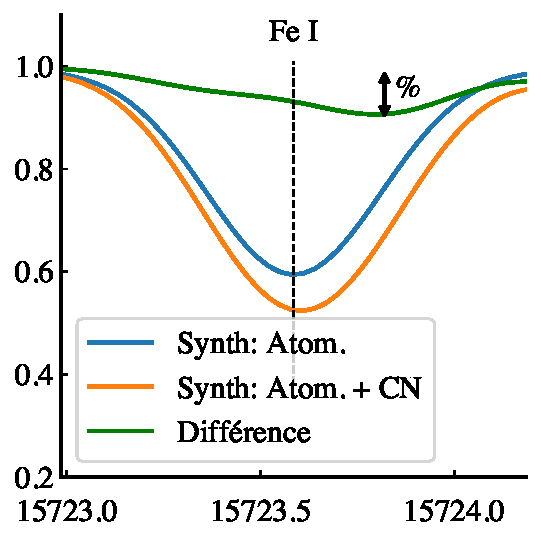
\includegraphics[width=4cm]{images/illu.pdf}
\end{column}
\end{columns}
    
\footnotesize{\textbf{Cat. III} ($<$ 1\%) : $^{13}$CH, $^{14}$NH, $^{48}$TiO, C$_{2}$H$_2$, HCl, $^{20}$CaH, $^{28}$SiH, $^{28}$SiO, VO, YO, $^{48}$TiO, $^{24}$MgH, AlH, $^{52}$CrH, H$^{12}$CN, H$^{13}$CN, $^{90-94}$ZrO et $^{96}$ZrO}

\end{frame}

% % \metroset{titleformat frame=allcaps}
% \begin{frame}[fragile]{Abondances C, N, O}

% Itération sur les abondances de C, N, O jusqu'à convergence

% \begin{table}[h!]
%       \vspace{0.3cm}
%     \begin{center}
%     	\begin{tabular}{ccccc}
%             \hline
%     		\hline
%             log $\varepsilon_{\rm O}$ & log $\varepsilon_{\rm C}$ & log $\varepsilon_{\rm N}$ & $^{12}$C/$^{13}$C & Raie\\
%             \hline
%             \cellcolor{blue!15}{8.59 $\pm$ 0.01} & 8.44 & 7.38 & 40 & $^{16}$OH \\
%         % % raie de bande H
%         8.59 & \cellcolor{blue!15}{7.82 $\pm$ 0.03} & 7.38 & 40 & $^{12}$C$^{16}$O \\
%         8.59 & 7.82 & 7.38 & \cellcolor{blue!15}{20} & $^{13}$C$^{17}$O \\
%         \cellcolor{blue!15}{8.30 $\pm$ 0.02} & 7.82 & 7.38 & 20 & $^{16}$OH \\
%         8.30 & \cellcolor{blue!15}{7.89 $\pm$ 0.02} & 7.38 & 20 & $^{12}$C$^{16}$O \\
%         \cellcolor{blue!15}{8.33 $\pm$ 0.02} & 7.89 & 7.38 & 20 & $^{16}$OH \\
%         8.33 & \cellcolor{blue!15}{7.86 $\pm$ 0.03} & 7.38 & 20 & $^{12}$C$^{16}$O \\
%         8.33 & 7.86 & \cellcolor{blue!15}{7.84 $\pm$ 0.02} & 20 & $^{12}$C$^{14}$N \\
%         8.33 & 7.86 & 7.84 & \cellcolor{blue!15}{12} & $^{13}$C$^{14}$N \\
%         \cellcolor{blue!15}{8.31 $\pm$ 0.01} & 7.86 & 7.84 & 12 & $^{16}$OH \\
%         8.31 & \cellcolor{blue!15}{7.88 $\pm$ 0.03} & 7.84 & 12 & $^{12}$C$^{16}$O \\
%         8.31 & 7.88 & \cellcolor{blue!15}{7.84 $\pm$ 0.02} & 12 & $^{12}$C$^{14}$N \\
%         \end{tabular}
%     \end{center} 
%     % \textbf{Notes.} 
%     % Chaque synthèse est réalisée sur des raies de l'élement se trouvant en 4ème colonne. 
%     % Les paramètres fixés sont en noir et le paramètre déterminé en bleu. 
%     % \label{itération_CNO_ancien}
%     \end{table}

% \end{frame}


\begin{frame}[fragile]{Abondances C, N, O}
    \begin{columns}
        \begin{column}{0.3\textwidth}
            \vspace{1cm}

            Itération sur les abondances de C, N, O jusqu'à convergence. 
            
            \vspace{2cm}
            \begin{table}[h!]
                \vspace{0.3cm}
              \begin{center}
                \resizebox{8cm}{!}{
                  \begin{tabular}{c|cccc}
                    %   \hline
                    %   \hline
                      &log $\varepsilon_{\rm O}$ & log $\varepsilon_{\rm C}$ & log $\varepsilon_{\rm N}$ & $^{12}$C/$^{13}$C\\
                      \hline
                      Initial&- & 8.44 & 7.38 & 40 \\
                    Final&8.31$\pm$ 0.01 & 7.88 $\pm$ 0.03 & 7.84 $\pm$ 0.02 & 12 \\
                  \end{tabular}}
              \end{center} 
              \end{table}
            

        \end{column}
        \begin{column}{0.7\textwidth}
            \tikzstyle{block} = [draw, rectangle, 
        minimum height=3em, minimum width=3em
        ]
        \tikzstyle{virtual} = [coordinate]
        \begin{tikzpicture}[>=stealth,auto, node distance=1cm]
            \node[block, fill=UnccOrange!30] (block1) {$^{16}$OH};
            \node[block, right=of block1, fill=UnccGold] (block2) {A(O)};
            \node[block, below=of block2, fill=UnccOrange!30] (block3) {$^{12}$C$^{16}$O};
            \node[block, right=of block3, fill=UnccGold] (block4) {A(C)};
            \node[block, below=of block4,fill=BrickRed!30] (block5) {$^{12}$C/$^{13}$C};
            \node[block, right=of block4,fill=UnccOrange!30] (block6) {$^{12}$C$^{14}$N};
            \node[block, below=of block6, fill=UnccGold] (block7) {A(N)};
            \node[block, below=of block7, fill=BrickRed!30] (block8) {$^{12}$C/$^{13}$C};
            
            \draw[->] (block1) -- (block2) ;
            \draw[->] (block2) -- (block3);
            \draw[->] (block3) -- (block4);
            \draw[->] ([xshift=-0.2cm]block4.south) -- ([xshift=-0.2cm]block5.north);
            \draw[->] ([xshift=0.2cm]block5.north) -- ([xshift=0.2cm]block4.south);
            \draw[->] (block4) -- (block6);
            \draw[->] (block6) -- (block7);
            \draw[->] ([xshift=-0.2cm]block7.south) -- ([xshift=-0.2cm]block8.north);
            \draw[->] ([xshift=0.2cm]block8.north) -- ([xshift=0.2cm]block7.south);

            % \coordinate (midpoint) at ((block1)!0.5!(block2));
            % \draw[->] (midpoint) -- ++(0,0.1);

            % Modification des deux dernières flèches pour qu'elles contournent
            \draw[->] (block7) -| ++(1.,5) -| (block1.north);
            \draw[->] (block4.north)-| ++(0,2.4) -| (block1.north);
        \end{tikzpicture}
        \end{column}
    \end{columns}
\end{frame}

\begin{frame}[fragile]{Paramètres stellaires}
\begin{table}[h!]
    \begin{center}
        \renewcommand{\arraystretch}{1.5}
        \begin{tabular}{c|ccc|c}
            Paramètre & Infrarouge &Visible& Littérature &Commentaires\\
            \hline
            % &&&\\
            % \arrayrulecolor{red}\hline
            % \multicolumn{1}{|c}{$[$Fe/H$]$ (dex)}& -0.25 $\pm$ 0.10 & -0.37 &
            % \multicolumn{1}{c|}{-0.30}\\
            % \arrayrulecolor{red}\hline
            $[$Fe/H$]$ [dex]& -0.25 $\pm$ 0.10 & -0.37 &-0.30$\pm$ 0.09&\\
            % \multicolumn{1}{c|}{-0.30}\\
            % &&&\\
            T$_{\rm eff}$ [K] & 4000 $\pm$ 125 &4307 & 4000& \\

            log $g$ [cm/s$^2$]& to do & 2.29 & 1.00&raies de Ti II\\
            % &&&\\
            log $g$  & 1.04 & 1.54 & 1.00 &isochrones\\
            % &&&\\
            log $g$  & to do & - & 1.00 &tracés évolutifs\\
            % &&\\
            log $g$  & 0.3$\pm$0.3 &-& 1.00 &ailes raies fortes\\
            %  &&\\
            $\xi_{\text{micro}}$ [km/s]& to do & to do & - &\\
            % &&&\\
        \end{tabular}
    \end{center}
\end{table}
\end{frame}

\begin{frame}[fragile]{Paramètres stellaires}
    \begin{table}[h!]
        \begin{center}
            \renewcommand{\arraystretch}{1.5}
            \begin{tabular}{c|ccc|c}
                Paramètre & Infrarouge &Visible& Littérature &Commentaires\\
                \hline
                % &&&\\
                % \arrayrulecolor{red}\hline
                % \multicolumn{1}{|c}{$[$Fe/H$]$ (dex)}& -0.25 $\pm$ 0.10 & -0.37 &
                % \multicolumn{1}{c|}{-0.30}\\
                % \arrayrulecolor{red}\hline
                \arrayrulecolor{red}\hline
                \multicolumn{1}{|c}{$[$Fe/H$]$ [dex]}& -0.25 $\pm$ 0.10 & -0.37 &
                -0.30$\pm$ 0.09&\multicolumn{1}{c|}{}\\
                \arrayrulecolor{red}\hline
                % \multicolumn{1}{c|}{-0.30}\\
                % &&&\\
                T$_{\rm eff}$ [K] & 4000 $\pm$ 125 &4307 & 4000& \\
    
                log $g$ [cm/s$^2$]& to do & 2.29 & 1.00&raies de Ti II\\
                % &&&\\
                log $g$  & 1.04 & 1.54 & 1.00 &isochrones\\
                % &&&\\
                log $g$  & to do & - & 1.00 &tracés évolutifs\\
                % &&\\
                log $g$  & 0.3$\pm$0.3 &-& 1.00 &ailes raies fortes\\
                %  &&\\
                $\xi_{\text{micro}}$ [km/s]& to do & to do & - &\\
                % &&&\\
            \end{tabular}
        \end{center}
    \end{table}
    \end{frame}

\begin{frame}[fragile]{Métallicité [Fe/H]}
    \begin{center}
        [Fe/H] = log $\varepsilon_{\mathrm{Fe_*}}$ - log $\varepsilon_{\mathrm{Fe_{\odot}}}$
        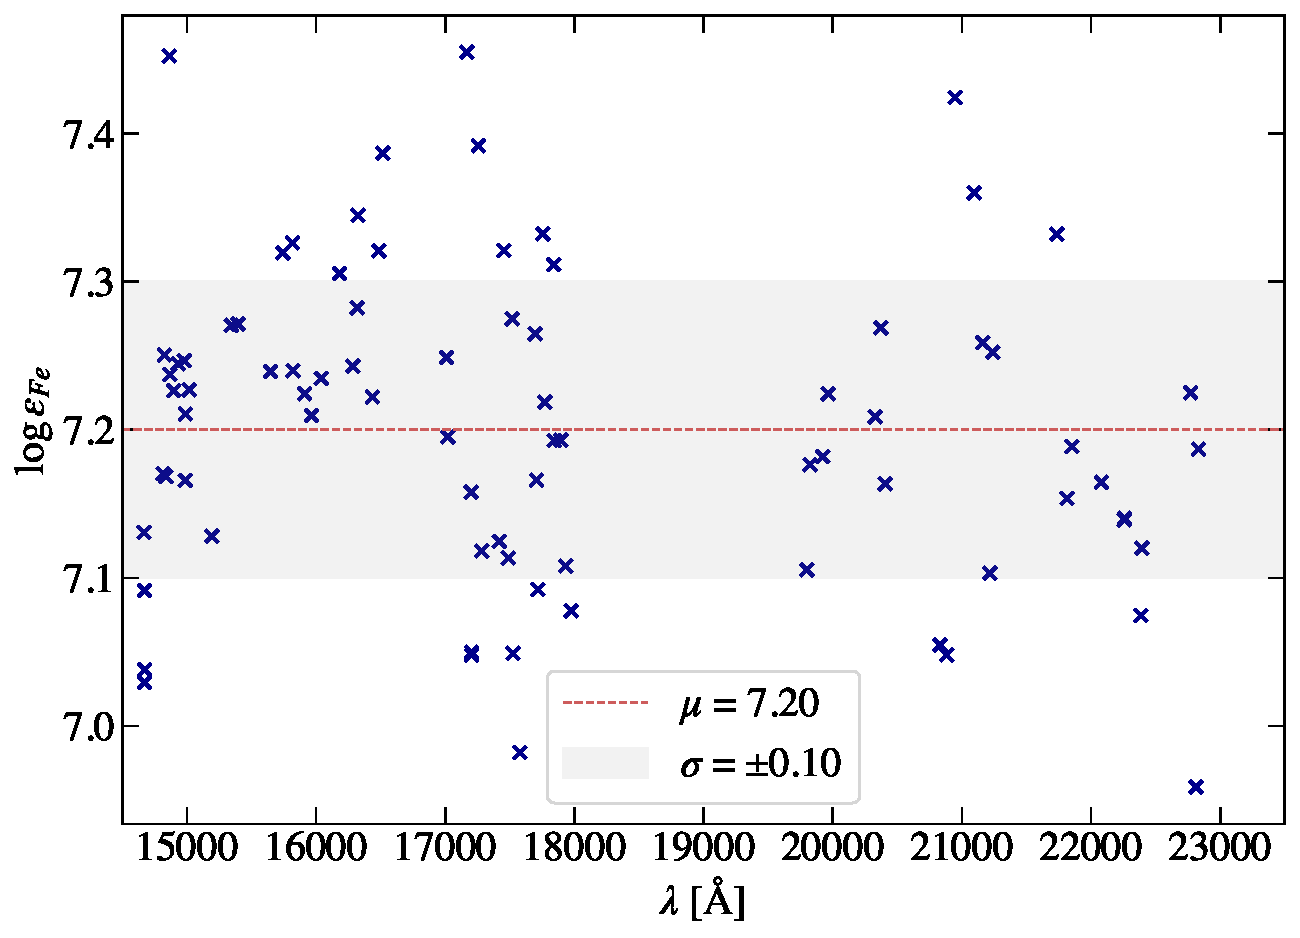
\includegraphics[width=10cm]{images/Fe_abu_4000.pdf}
    \end{center}
\end{frame}


\begin{frame}[fragile]{Paramètres stellaires}
    \begin{table}[h!]
        \begin{center}
            \renewcommand{\arraystretch}{1.5}
            \begin{tabular}{c|ccc|c}
                Paramètre & Infrarouge &Visible& Littérature &Commentaires\\
                \hline
                % &&&\\
                % \arrayrulecolor{red}\hline
                % \multicolumn{1}{|c}{$[$Fe/H$]$ (dex)}& -0.25 $\pm$ 0.10 & -0.37 &
                % \multicolumn{1}{c|}{-0.30}\\
                % \arrayrulecolor{red}\hline
                
                $[$Fe/H$]$ [dex]& -0.25 $\pm$ 0.10 & -0.37 &
                -0.30$\pm$ 0.09&\\
                % \multicolumn{1}{c|}{-0.30}\\
                % &&&\\
                \arrayrulecolor{red}\hline
                \multicolumn{1}{|c}{T$_{\rm eff}$ [K]} & 4000 $\pm$ 125 &4307 & 4000& \multicolumn{1}{c|}{}\\
                \arrayrulecolor{red}\hline
    
                log $g$ [cm/s$^2$]& to do & 2.29 & 1.00&raies de Ti II\\
                % &&&\\
                log $g$ & 1.04 & 1.54 & 1.00 &isochrones\\
                % &&&\\
                log $g$ & to do & - & 1.00 &tracés évolutifs\\
                % &&\\
                log $g$  &0.3$\pm$0.3 &-& 1.00 &ailes raies fortes\\
                %  &&\\
                $\xi_{\text{micro}}$ [km/s]& to do & to do & - &\\
                % &&&\\
            \end{tabular}
        \end{center}
    \end{table}
    \end{frame}


\begin{frame}[fragile]{Température effective}
    Respect de l'équation de Boltzmann $\rightarrow$  abondance d'un élément ne varie pas en fonction du potentiel d'excitation \\ 
    % $$\frac{\mathrm{n}_\mathrm{i}}{\mathrm{N}}=\frac{\mathrm{g}_\mathrm{i}}{\mathrm{U(T)}} \ e^{-\chi_\mathrm{i}/\mathrm{kT}}$$
    \vspace{1cm}
    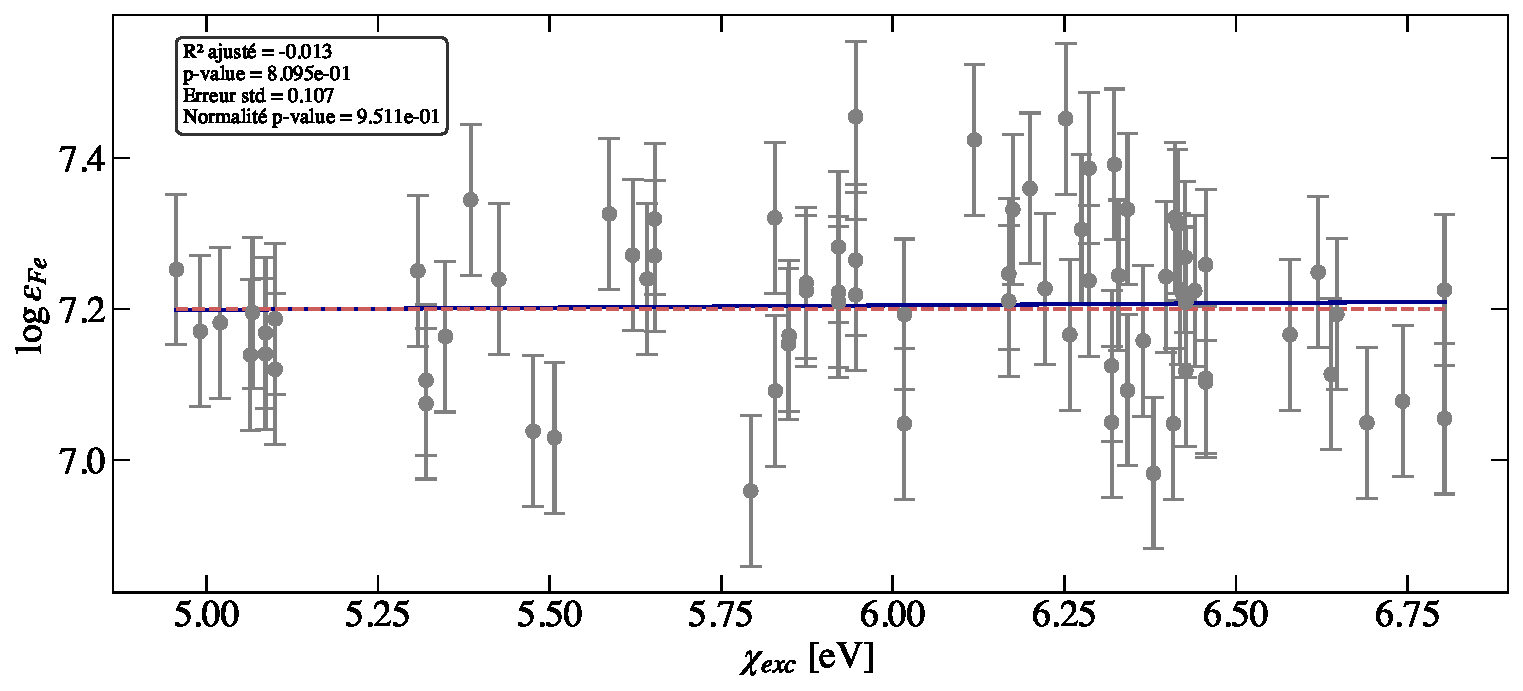
\includegraphics[width=\textwidth]{images/comparaison_modèles.pdf}
\end{frame}

\begin{frame}[fragile]{Paramètres stellaires}
    \begin{table}[h!]
        \begin{center}
            \renewcommand{\arraystretch}{1.5}
            \begin{tabular}{c|ccc|c}
                Paramètre & Infrarouge &Visible& Littérature &Commentaires\\
                \hline
                % &&&\\
                % \arrayrulecolor{red}\hline
                % \multicolumn{1}{|c}{$[$Fe/H$]$ (dex)}& -0.25 $\pm$ 0.10 & -0.37 &
                % \multicolumn{1}{c|}{-0.30}\\
                % \arrayrulecolor{red}\hline
                
                $[$Fe/H$]$ [dex]& -0.25 $\pm$ 0.10 & -0.37 &
                -0.30$\pm$ 0.09&\\
                % \multicolumn{1}{c|}{-0.30}\\
                % &&&\\
                T$_{\rm eff}$ [K] & 4000 $\pm$ 125 &4307 & 4000& \\
    
                log $g$ [cm/s$^2$]& to do & 2.29 & 1.00&raies de Ti II\\
                % &&&\\
                \arrayrulecolor{red}\hline
                \multicolumn{1}{|c}{log $g$ }& 1.04 & 1.54 & 1.00 &\multicolumn{1}{c|}{isochrones}\\
                  \arrayrulecolor{red}\hline
                % &&&\\
                log $g$ & to do & - & 1.00 &tracés évolutifs\\
                % &&\\
                log $g$ & 0.3$\pm$0.3 &-& 1.00 &ailes raies fortes\\
                %  &&\\
                $\xi_{\text{micro}}$ [km/s]& to do & to do & - &\\
                % &&&\\
            \end{tabular}
        \end{center}
    \end{table}
    \end{frame}

\begin{frame}[fragile]{Gravité de surface : isochrones}
    \begin{columns}
        \begin{column}{0.3\textwidth}
            Isochrone du code PARSEC (code d'évolution stellaire). \\
            \vspace{0.5cm}
            Amas d'étoiles de même âge, supposé ici à 1-10 Gyr. 
        \end{column}
        \begin{column}{0.7\textwidth}
            \begin{center}
                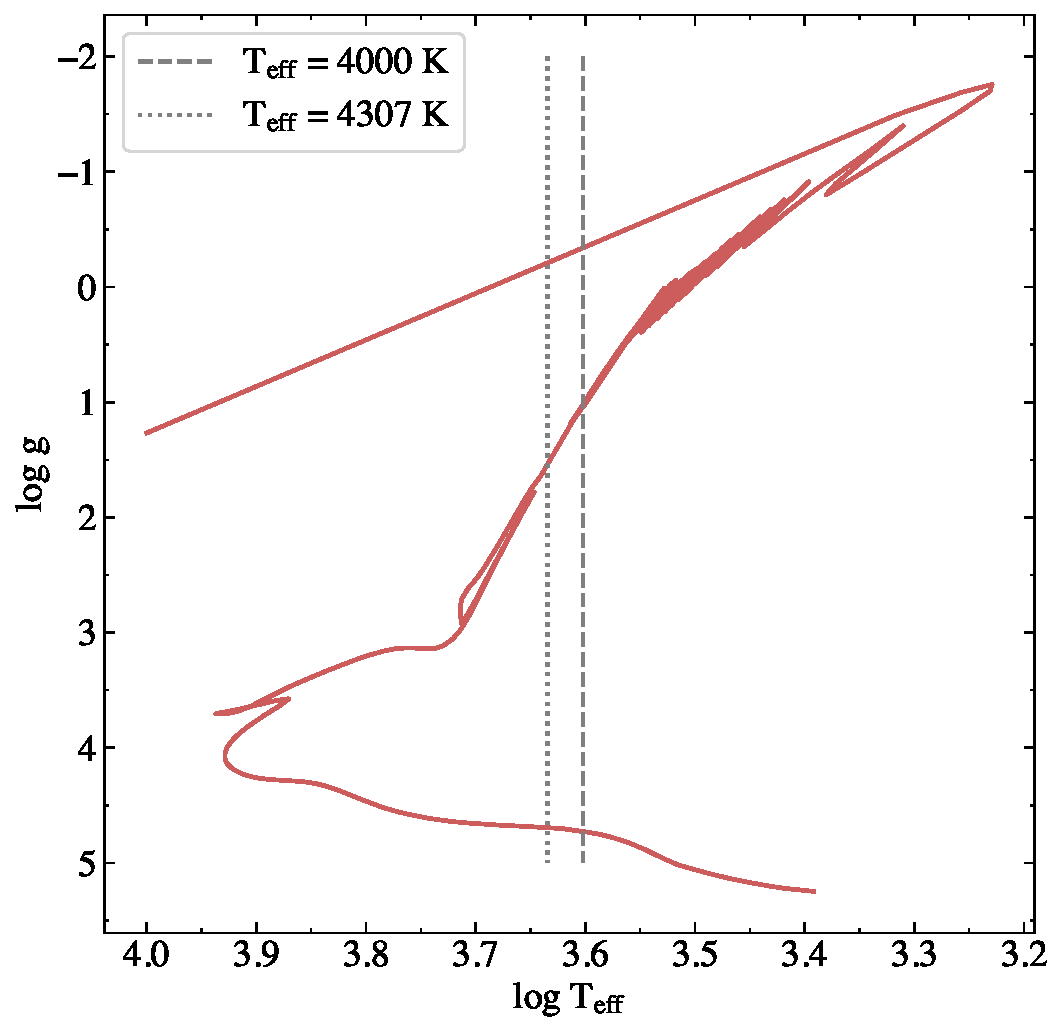
\includegraphics[width=8cm]{images/isochrones.pdf}
            \end{center}
            
        \end{column}
    \end{columns}
\end{frame}

\begin{frame}[fragile]{Paramètres stellaires}
    \begin{table}[h!]
        \begin{center}
            \renewcommand{\arraystretch}{1.5}
            \begin{tabular}{c|ccc|c}
                Paramètre & Infrarouge &Visible& Littérature &Commentaires\\
                \hline
                % &&&\\
                % \arrayrulecolor{red}\hline
                % \multicolumn{1}{|c}{$[$Fe/H$]$ (dex)}& -0.25 $\pm$ 0.10 & -0.37 &
                % \multicolumn{1}{c|}{-0.30}\\
                % \arrayrulecolor{red}\hline
                
                $[$Fe/H$]$ [dex]& -0.25 $\pm$ 0.10 & -0.37 &
                -0.30$\pm$ 0.09&\\
                % \multicolumn{1}{c|}{-0.30}\\
                % &&&\\
                T$_{\rm eff}$ [K] & 4000 $\pm$ 125 &4307 & 4000& \\
    
                log $g$ [cm/s$^2$]& to do & 2.29 & 1.00&raies de Ti II\\
                % &&&\\
                log $g$ & 1.04 & 1.54 & 1.00 &isochrones\\
                  
                % &&&\\
                log $g$ & to do & - & 1.00 &tracés évolutifs\\
                % &&\\
                \arrayrulecolor{red}\hline
                \multicolumn{1}{|c}{log $g$ }& 0.3$\pm$0.3 & 1.54 & 1.00 &\multicolumn{1}{c|}{ailes de raies fortes}\\
                \arrayrulecolor{red}\hline
                %  &&\\
                $\xi_{\text{micro}}$ [km/s]& to do & to do & - &\\
                % &&&\\
            \end{tabular}
        \end{center}
    \end{table}
    \end{frame}

\begin{frame}[fragile]{Gravité de surface : ailes de raies fortes}
   \begin{columns}
       \begin{column}{0.3\textwidth}
        Minimisisation $\chi^2$ sur ailes de raies fortes de Mg I et Ca I.
       \end{column}
       \begin{column}{0.7\textwidth}
           \begin{center}
            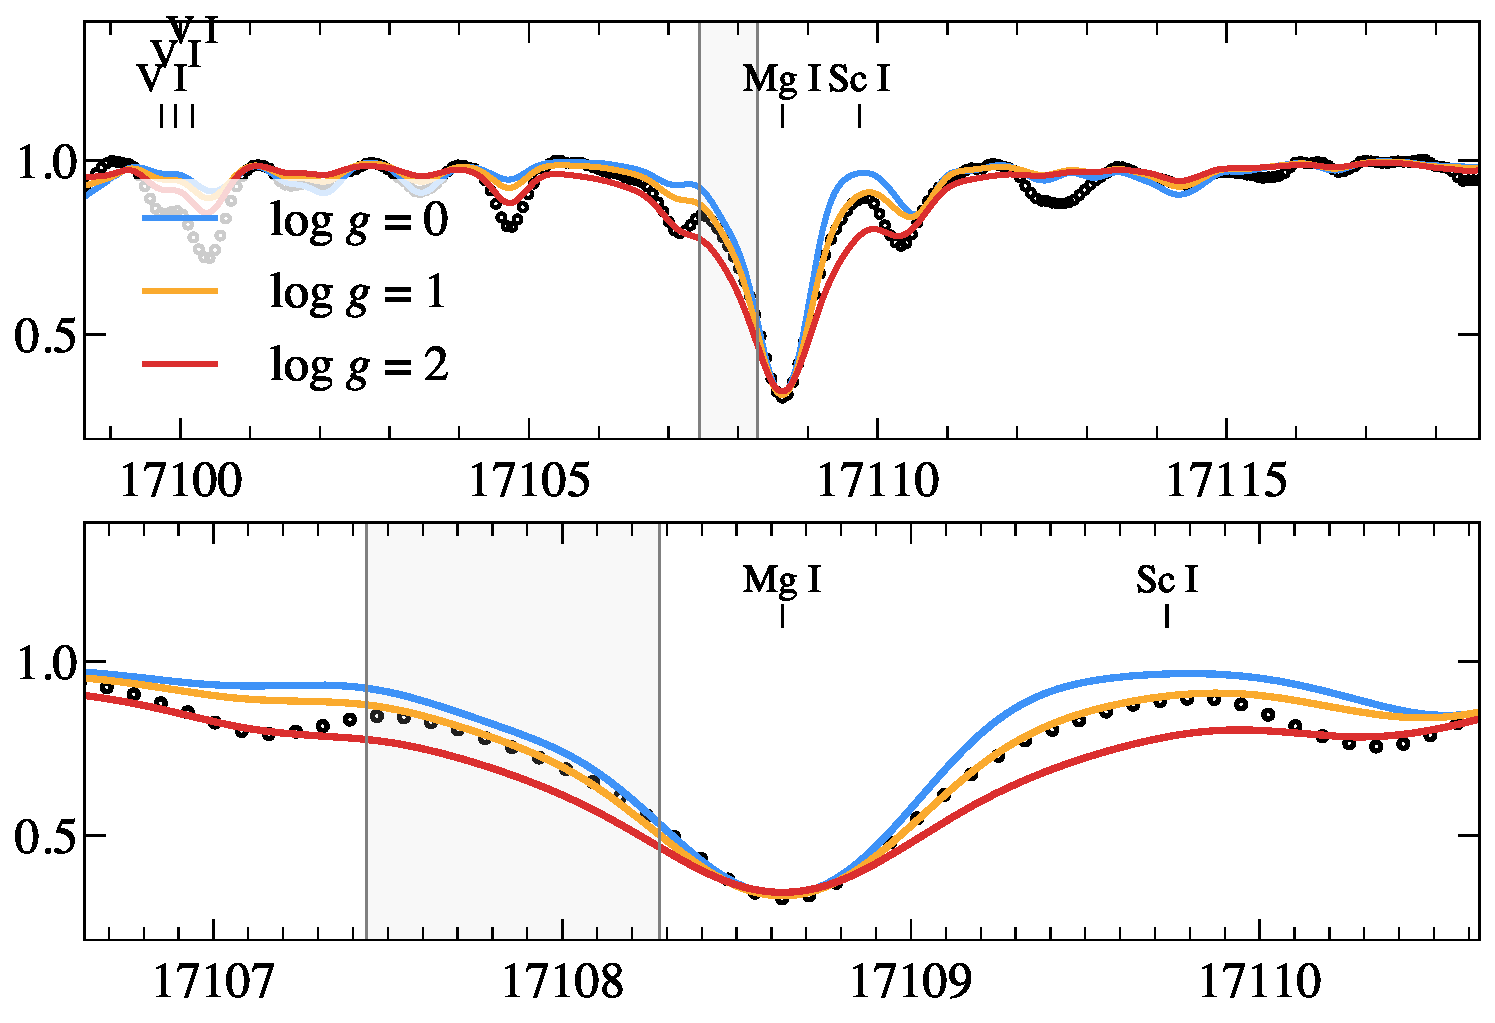
\includegraphics[width=8cm]{images/test4.pdf}  
           \end{center}
       \end{column}
       \end{columns}
\end{frame}

\begin{frame}[fragile]{Paramètres stellaires}
    \begin{table}[h!]
        \begin{center}
            \renewcommand{\arraystretch}{1.5}
            \begin{tabular}{c|ccc|c}
                Paramètre & Infrarouge &Visible& Littérature &Commentaires\\
                \hline
                % &&&\\
                % \arrayrulecolor{red}\hline
                % \multicolumn{1}{|c}{$[$Fe/H$]$ (dex)}& -0.25 $\pm$ 0.10 & -0.37 &
                % \multicolumn{1}{c|}{-0.30}\\
                % \arrayrulecolor{red}\hline
                
                $[$Fe/H$]$ [dex]& -0.25 $\pm$ 0.10 & -0.37 &
                -0.30$\pm$ 0.09&\\

                % \multicolumn{1}{c|}{-0.30}\\
                % &&&\\
                T$_{\rm eff}$ [K] & 4000 $\pm$ 125 &4307 & 4000& \\
    
                \rowcolor{gray!15} log $g$ [cm/s$^2$]& to do & 2.29 & 1.00&raies de Ti II\\
                % &&&\\
                log $g$  & 1.04 & 1.54 & 1.00 &isochrones\\
                % &&&\\
                \rowcolor{gray!15}log $g$  & to do & - & 1.00 &tracés évolutifs\\
                % &&\\
                log $g$ & 0.31 &-& 1.00 &ailes raies fortes\\
                %  &&\\
                \rowcolor{gray!15} $\xi_{\text{micro}}$ [km/s]& to do & to do & - &\\
                % &&&\\
            \end{tabular}
        \end{center}
    \end{table}
    \end{frame}

\begin{frame}[fragile]{Autres paramètres}
    \begin{columns}
        \begin{column}{0.48\textwidth}
            \begin{center}
                \textbf{Gravité de surface}
               \begin{itemize}
                \item [-] Respect de l'équation de Saha  $\rightarrow$ abondance identique pour l'élément neutre et ses différents états d'ionisation (raies de Ti II)
                \item [-] Tracés évolutifs (estimer masse)
               \end{itemize}
            \end{center}
        \end{column}
        \begin{column}{0.04\textwidth}
            \begin{tikzpicture}
                \draw[thick] (0,-1) -- (0,5);
            \end{tikzpicture}
        \end{column}
        \begin{column}{0.48\textwidth}
            \begin{center}
                \textbf{Microturbulence}  
                \begin{itemize}
                    \item [-] Paramètre \textit{ad hoc}, permet de modéliser les effets de turbulence à des échelles plus petites que le libre parcours moyen des photons
                    \item [-] Abondance ne varie pas en fonction de la largeur équivalente réduite
                \end{itemize}
            \end{center}
        \end{column}

\end{columns}
\end{frame}
 

\begin{frame}[fragile]{Raies atomiques}
    % Ca I, Mg I, Al I, Si I, K I, Sc I, Ti I, Ti II, V I, Mn I, Fe I, Co I, Ni I, Cu I, Y I, Zr I, Ba I, Ce II, Ce III, Er II, Yb II

% % \begin{column}{0.5\textwidth}
        \begin{table}[h!]
            \begin{center}
                \begin{tabular}{c|c|c}
                     & Élement & Nb. raies\\
                    \hline
                    Pic du fer & Sc I &115\\
                     & Ti I&63\\
                     & Ti II&7\\
                     & V I&76\\
                     & Cr I&20\\
                     & Mn I&55\\
                     &Fe I&81\\
                    & Co I&69\\
                    & Ni I&58\\
                    $\alpha$ & Mg I&12\\
                     & Si I&13\\
                     & Ca I& 5\\
                \end{tabular}
            \end{center}
        \end{table}
% %     \end{column}
% %     \begin{column}{0.5\textwidth}
% %         \begin{table}[h!]
% %             \begin{center}
% %                 \begin{tabular}{c|c|c}
% %                      & Élement & Nb. raies\\
% %                     \hline
% %                     &&\\
% %                     Z impaire & Na I &19\\
% %                      & Al I &7\\
% %                      & K I &5 \\
% %                     s & Cu I & 5\\
% %                      & Y I & 17\\
% %                      & Zr I & 2\\
% %                      & Ba I & 2\\
% %                      & Ce II & 9\\
% %                      & Ce III & 2\\
% %                      & Nd II & 7\\
% %                      & Yb II & 2\\
% %                 \end{tabular}
% %             \end{center}
% %         \end{table}
% %     \end{column}
% \end{colums}
\end{frame}
\begin{frame}[fragile]{Raies atomiques suite}
            \begin{table}[h!]
            \begin{center}
                \begin{tabular}{c|c|c}
                     & Élement & Nb. raies\\
                    \hline
                    Z impair & Na I &19\\
                     & Al I &7\\
                     & K I &5 \\
                    s & Cu I & 5\\
                     & Y I & 17\\
                     & Zr I & 2\\
                     & Ba I & 2\\
                     & Ce II & 9\\
                     & Ce III & 2\\
                     & Nd II & 7\\
                     & Yb II & 2\\
                \end{tabular}
            \end{center}
        \end{table}
\end{frame}

\begin{frame}[fragile]{La suite ?}
    \begin{itemize}
        \item finir détermination paramètres stellaires
        \item comparaison avec abondances déterminées dans le visible à partir de spectre HERMES
        \item détermination  d'abondances d'éléments lourds ETL et non-ETL
        \begin{itemize}
            \item [-] besoin de listes non-ETL
            \item [-] besoin d'interpoler modèles et coefficients d'écarts non-ETL
        \end{itemize}
        \item comparaison profil d'abondances avec modèles de nucléosynthèse
    \end{itemize} 
\end{frame}

% \begin{frame}[fragile]{Slide supplémentaire}
%     suppe
% \end{frame}

% \begin{frame}[fragile]{Micro \& Macroturbulence}
%     macro
% \end{frame}

% \begin{frame}[fragile]{Méthode Feautrier}
%     feautrier
% \end{frame}

% \begin{frame}[fragile]{Profil de Voigt}
% élargissement naturel des raies du à incertitude sur l'énergie des transitions -> profil de Lorentz de paramètre $\gamma^{rad}$

% élargissement du aux collisons, quand on utilise approximation d'impact (pertubateur arrive à grande vitesse et cause perturbation momentannée du train d'onde émis par atome excité) -> profil de Lorentz de paramètre $\gamma^{coll}$

% --> convolution de deux profils de lorentz donne un profil de lorentz de $\gamma$ = $\gamma^{rad}$ + $\gamma^{coll}$
% \end{frame}

% \begin{frame}[fragile]{Effet Stark linéaire}
%     collisons 
% \end{frame}

% \begin{frame}[fragile]{Théorie ABO}
%     abo
% \end{frame}

\begin{frame}[fragile]{Mécanisme de production dans AGB}
    \begin{columns}
        \begin{column}{0.3\textwidth}
            Instabilités thermiques durant combustion de la couche He $\rightarrow$ réajustement, engloutissement enveloppe convective. \\
            \vspace{2cm}
            Source neutronique : \\
            $^{12}$C(p,$\gamma$)$^{13}$N($\beta^+$)$^{13}$C($\alpha$,\textcolor{red}{n})$^{16}$O \\
             $^{22}$Ne($\alpha$,\textcolor{red}{n})$^{25}$Mg      
        \end{column}
        \begin{column}{0.7\textwidth}
            \begin{center}
                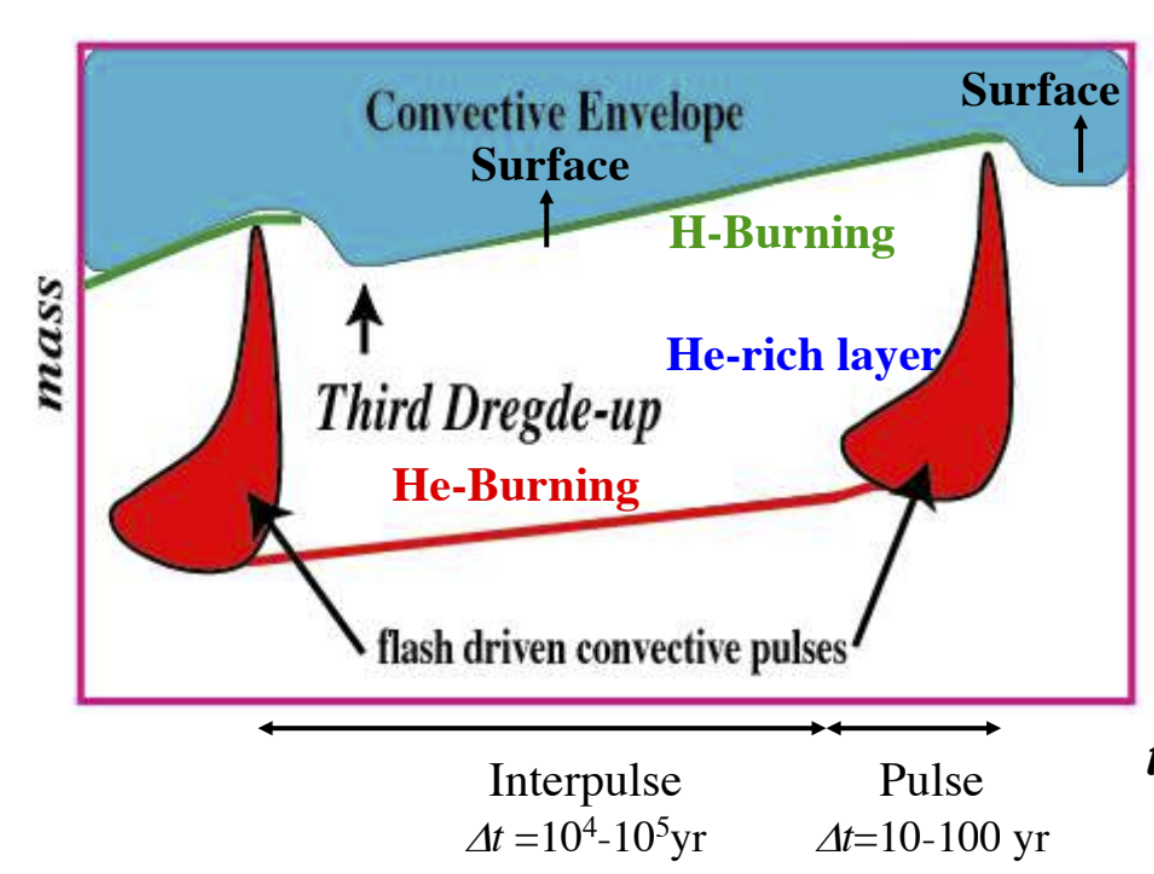
\includegraphics[width=8cm]{images/pmz.png}
                \vspace{2cm}
            \end{center}
        \end{column}
    \end{columns}
\end{frame}

\end{document}
